\chapter{Object level vision}
\minitoc


\section{General factor}
Let's assume that an algorithm provides us $\Tm{C}{O} \in \SE(3)$, a measurement the pose of an element 
of the scene with an attached frame $O$ with respect to the camera frame $C$ located at the Camera optical frame.
The kinematic chain of the problem described in \figRef{fig:camera_object_chain} unrolls as 
$\T{W}{O} = \T{W}{B}\T{B}{C}\T{C}{O}$ where W and B correspond to the world and body frames.
Given measurement $\Tm{C}{O}$, this relation can therefore be turned into a residual relating 
the robot pose, the camera extrinsics and the object pose:

\begin{equation}
    \bfr (\T{W}{B}, \T{B}{C}, \T{W}{O}) = \Log(\T{W}{O} \T{W}{B}^{-1} \T{B}{C}^{-1} \T{C}{O}^{-1}) ~ \in \Reals^6
\end{equation}

We also assume that we have access to the covariance of this measurement 
$\Cov_V \in \Reals^{6 \times 6}$. We will now describe two applications of this factor, one using Apriltag fiducial markers and one using 
a Deeplearning object pose estimation algorithm.

\begin{figure}
    \centering
    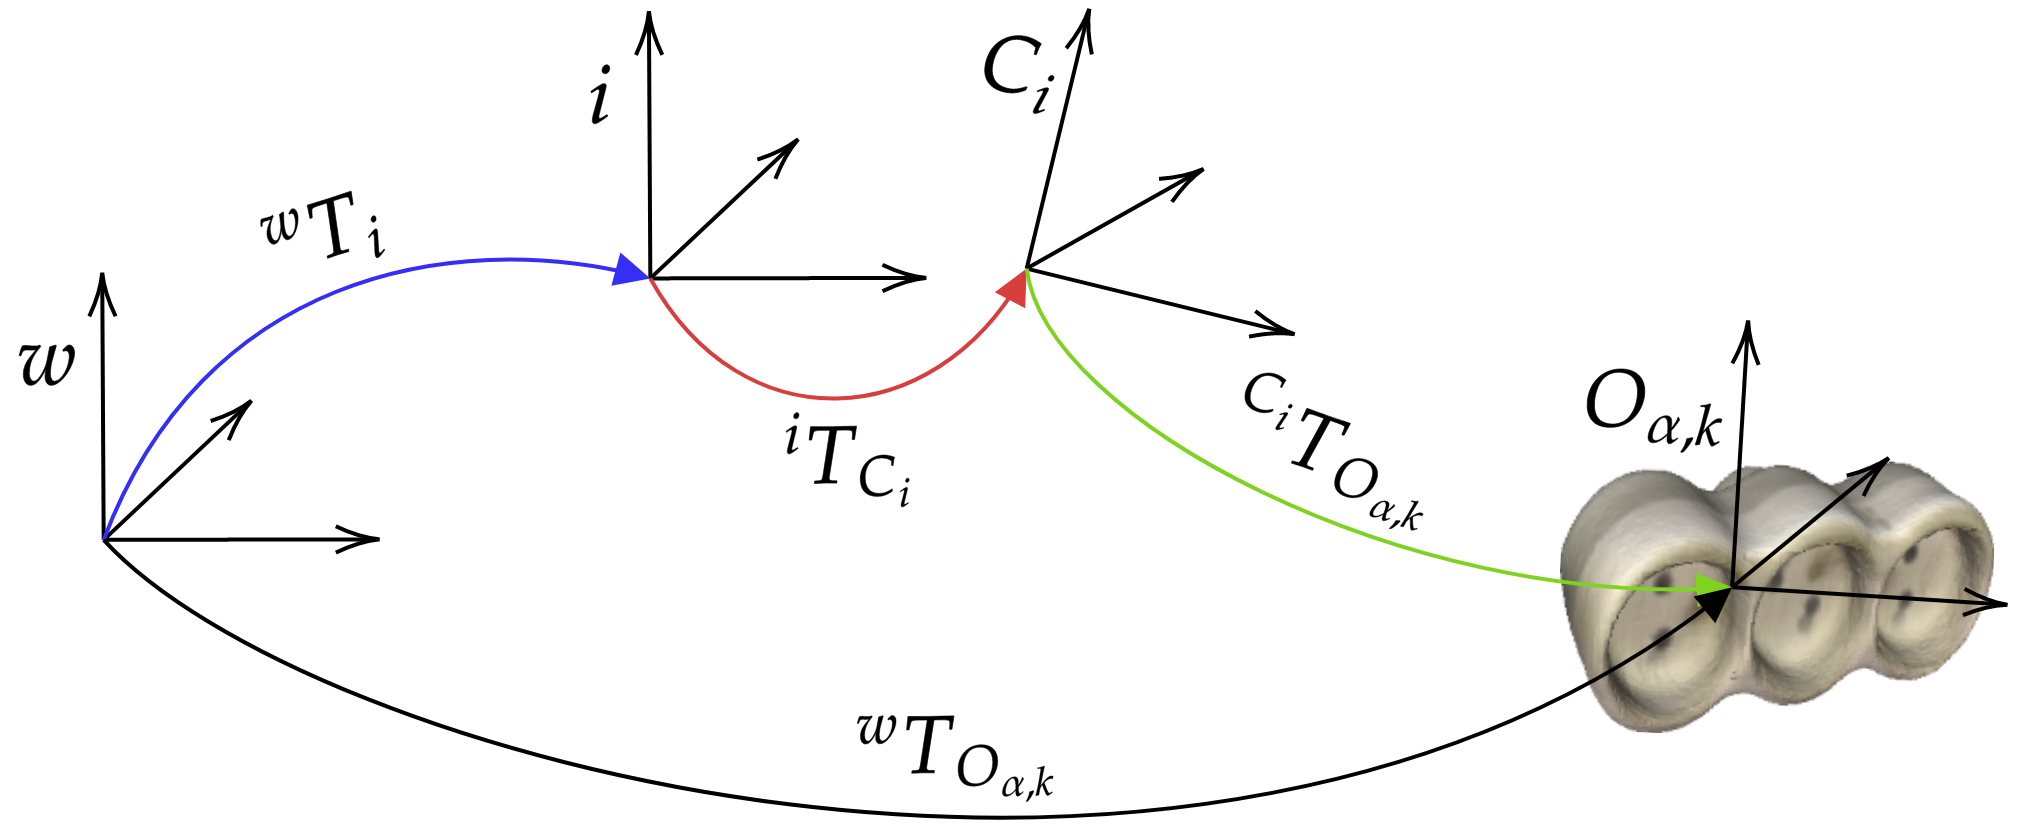
\includegraphics[width=0.7\textwidth]{figures/fig_kinematic_Cesar.png}
    \caption{Camera/object kinematic chain from ICRA paper, to replace }
    \label{fig:camera_object_chain}
\end{figure}

\section{Fiducial marker}
\subsection{Markers Pose estimation algorithms}
Sota on the question
Apriltag: \cite{wang2016iros}
IPPE: \cite{collins2014infinitesimal}

\subsection{Covariance model}
Appart from designing more precise and more efficient algorithm for fiducial marker detection and specialized PnP algorithms,
 obtain covariances from these prediction has been the focus of a series of papers.
 SOTA

Instead of directly obtaining Jacobians from the PnP algorithms, we found that a natural way to proceed is to take the opposite 
direction. It should somehow be possible, knowing the marker size and the relative pose measurement, and assuming pixel noise, to
recover $\Cov_{OV}$. A simple model of this noise is to assume isotropic Gaussian noise on the pixels. If we stack four pixel (the four tag corners) 
$\bfx_i = [u_i, v_i] \in \Reals^2$ and we stack then in the vector $\bfx = [\bfx_1 \bfx_2 \bfx_3 \bfx_4]$, we have therefore that
$\bfx$ is corrupted by a Gaussian noise $\Cov_{\bfx} = \sigma_{x}^2 \bfI$, where $\sigma_{x}$ usually takes values of 1 or 2 pixels.
PnP algorithm provides us with a function $pnp$ defined as:

\begin{equation}
    \begin{split}
        f: \Reals^8 &\rightarrow SE(3) \\
                           \bfx &\rightarrow \T{C}{O} = pnp_w(\bfx)
    \end{split}
\end{equation}

where w denotes the dependency on the width of the marker. This $pnp_w$ function implementation depends on the specificities of the PnP algorithm used and  
is in general hard to differentiate. Instead if we consider the inverse function

\begin{equation}
    \begin{split}
        g: SE(3) &\rightarrow \Reals^8 \\
                           \T{C}{O} &\rightarrow \bfx = proj_w(\T{C}{O})
    \end{split}
\end{equation}

that maps the relative pose to the projection of the tag in the image, a rather simple jacobian expression can be derived using the chain rule, as follows.

Let's defined the marker corner coordinates in the marker frame, like shown in \fig \figRef{fig:tag_coordinate_frame}. As a convention 
\cite{wang2016iros} we order the corners counter-clockwise starting from bottom left (looking straight at the tag). 

\begin{equation}
    c =
    \begin{pmatrix}
    c_1 \\ c_2 \\ c_3 \\ c_4
    \end{pmatrix}
    ~~
    c_1 =  \begin{pmatrix} -\frac{w}{2} \\ \frac{w}{2} \\ 0 \end{pmatrix}
    ~ 
    c_2 =  \begin{pmatrix} \frac{w}{2} \\ \frac{w}{2} \\ 0 \end{pmatrix}
    ~
    c_3 =  \begin{pmatrix} \frac{w}{2} \\ -\frac{w}{2} \\ 0 \end{pmatrix}
    ~
    c_4 =  \begin{pmatrix} -\frac{w}{2} \\ -\frac{w}{2} \\ 0 \end{pmatrix}
\end{equation}.

%
\begin{figure}
    \centering
    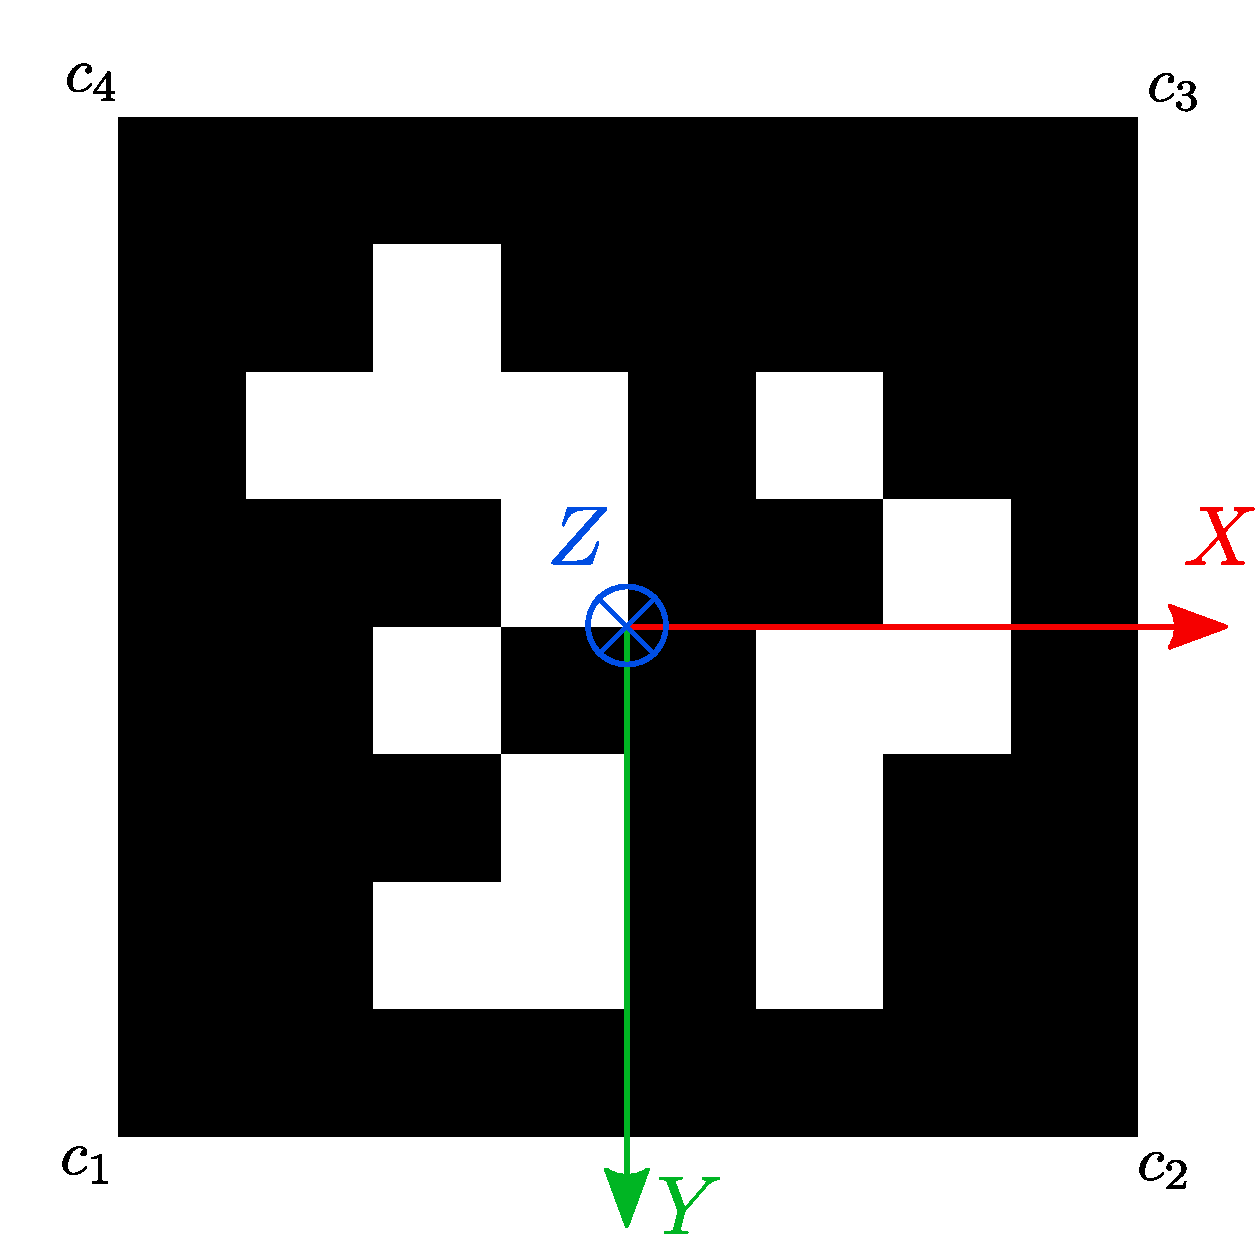
\includegraphics[width=0.5\textwidth]{figures/tag12_frame.pdf}
    \caption{Apriltag local coordinate systems and corners conventions \cite{wang2016iros}}
    \label{fig:tag_coordinate_frame}
\end{figure}

Then, assuming that images are corrected (no distortion), the pinpoint camera model gives us that

\begin{equation}
    \bfx_i = eucl(h_i) = eucl(K\T{C}{O} c_i)
\end{equation}
for each corner $c_i$, where $h_i$ are the homogeneous coordinates representing the projected corners and $eucl$ is the euclideanization function defined as
\begin{equation}
    \begin{split}
        eucl: \Reals^3 &\rightarrow \Reals^2 \\
        h = \begin{pmatrix}x\\y\\z\end{pmatrix} &\rightarrow \bfx = \begin{pmatrix}x/z\\y/z\end{pmatrix}
    \end{split}
\end{equation}

We need to compute the jacobian of each corner projection with respect to the estimated relative pose $J^{x_i}_{\T{}{}} = J^{x_i}_{h_i} J^{h_i}_{\T{}{}}$. 
Regarding the transformation, we will consider it to be an element of $\Reals(3)\times \SO(3)$ since the translation and rotation part 
of transformation are treated separately in our solver. The expressions of those functions are therefore expressed as:

% DROP dependency on C L for clearer notation?
\begin{equation}
    \begin{split}
        &h_i = K(\Rot{C}{O}c_i + \posi{C}{O}) \\
        &J^{h_i}_{\posi{C}{O}} = K ~~~~~~ J^{h_i}_{\Rot{C}{O}} = -K\Rot{C}{O}[c_i]_{\times}  \\  
        &J^{h_i}_{\T{C}{O}} = [J^{h_i}_{\posi{C}{O}} ~J^{h_i}_{\Rot{C}{O}}] = K [I_3 ~~~ -\Rot{C}{O} [c_i]_{\times}]
    \end{split}
\end{equation}
while the euclideanization jacobian is found to be
\begin{equation}
    J^{x_i}_{h_i}
    =
    \begin{pmatrix}
    1/z_i & 0 & -x_i/z_i^2 \\
    0 & 1/z_i & -y_i/z_i^2
    \end{pmatrix}
\end{equation}


Finally, we can stack the 4 jacobians to get the full jacobian to be used for covariance propagation.
\begin{equation}
    J \triangleq J^{\bfx}_{\T{C}{O}}=
    \begin{pmatrix}
    J^{\bfx_1}_{\T{C}{O}} \\ J^{\bfx_2}_{\T{C}{O}} \\ J^{\bfx_3}_{\T{C}{O}} \\ J^{\bfx_4}_{\T{C}{O}}
    \end{pmatrix}
    ~ \in \Reals^{8 \times 6}
\end{equation}.. 


We therefore have the covariance propagation equation $Q_{\bfx} = J Q_{\T{C}{O}} J^T$. 
This equation must be inverted in order to recover the needed covariance. $J$ being non square, 
we have to use the pseudo inverse to write: $\Cov_{\T{C}{O}} = J^{T,\dagger} \Cov_{\bfx} J^{\dagger}$. 
Knowing that the pixel noise covariance is isotropic as explained above, this equation simplifies to:

\begin{equation}
Q_{\T{C}{O}} = \sigma_{\bfx}^2(J^T J)^{-1}    
\end{equation}

Note that the derivations above are not limited to a square tag with four corners and could in theory be used for any object defined as
a set of point in its local coordinate system.





\section{Object pose estimation}
\subsection{Learning based single view object pose estimation}
Small sota + general cosypose workings
\subsection{Empirical covariance estimation}
blabla